% INFO-H410 — Presentation Groupe 9
\documentclass{beamer}
\usetheme{Madrid}
\usepackage{xcolor}

% Blue palette — three shades
\definecolor{darkblue}{RGB}{10,  50, 100}
\definecolor{medblue} {RGB}{30, 100, 180}
\definecolor{lightblue}{RGB}{210, 228, 245}

% Override all Madrid colours
\setbeamercolor{palette primary}   {bg=darkblue,  fg=white}
\setbeamercolor{palette secondary} {bg=medblue,   fg=white}
\setbeamercolor{palette tertiary}  {bg=darkblue,  fg=white}
\setbeamercolor{palette quaternary}{bg=darkblue,  fg=white}
\setbeamercolor{structure}         {fg=darkblue}
\setbeamercolor{section in toc}    {fg=darkblue}
\setbeamercolor{titlelike}         {bg=darkblue,  fg=white}
\setbeamercolor{frametitle}        {bg=darkblue,  fg=white}

% Blocks — blue shades only 
\setbeamercolor{block title}         {bg=medblue,  fg=white}
\setbeamercolor{block body}          {bg=lightblue, fg=black}
\setbeamercolor{block title alerted} {bg=darkblue,  fg=white}
\setbeamercolor{block body alerted}  {bg=lightblue, fg=black}
\setbeamercolor{block title example} {bg=medblue,   fg=white}
\setbeamercolor{block body example}  {bg=lightblue, fg=black}
\setbeamercolor{alerted text}        {fg=medblue}
\setbeamercolor{itemize item}        {fg=medblue}
\setbeamercolor{itemize subitem}     {fg=darkblue}

\usepackage{amsmath,amssymb}
\usepackage{booktabs}
\usepackage{multirow}
\usepackage{graphicx}
\usepackage{url}

% Footline: wider author box, narrower page-number box
\makeatletter
\setbeamertemplate{footline}{%
  \leavevmode%
  \hbox{%
    \begin{beamercolorbox}[wd=.50\paperwidth,ht=2.25ex,dp=1ex,center]{palette primary}%
      \usebeamerfont{author in head/foot}\insertshortauthor%
    \end{beamercolorbox}%
    \begin{beamercolorbox}[wd=.42\paperwidth,ht=2.25ex,dp=1ex,center]{palette secondary}%
      \usebeamerfont{title in head/foot}\insertshorttitle%
    \end{beamercolorbox}%
    \begin{beamercolorbox}[wd=.08\paperwidth,ht=2.25ex,dp=1ex,right]{palette tertiary}%
      \usebeamerfont{date in head/foot}\insertframenumber\,/\,\inserttotalframenumber\hspace*{1.5ex}%
    \end{beamercolorbox}}%
  \vskip0pt%
}
\makeatother

\title{Automated University Course Scheduling}
\subtitle{A Comparative Study of CSP, Local Search, and Q-Learning}
\author{N.~Machichi \and U.~Nkwinga \and B.~Sogutlu \and G.~Van den Eynde}
\institute{Groupe 9 \quad MA1 Ing\'enieur Civil, ULB \\[4pt] INFO-H410 - Techniques of Artificial Intelligence, 2025-2026}
\date{}

\begin{document}

\begin{frame}
    \titlepage
\end{frame}

\begin{frame}{Outline}
    \tableofcontents
\end{frame}

% -------------------------------------------------------
\section{Problem Formulation}

\begin{frame}{University Course Scheduling}
    \textbf{Goal:} assign each course a (room, timeslot) pair that satisfies all constraints.

    \bigskip
    \textbf{Hard constraints} (must all hold):
    \begin{itemize}
        \item[\textbf{H1}] No professor teaches two simultaneous courses
        \item[\textbf{H2}] No room hosts two simultaneous courses
        \item[\textbf{H3}] Room capacity $\geq$ course required capacity
        \item[\textbf{H4}] Timeslot $\in$ professor's availability
    \end{itemize}

    \bigskip
    \textbf{Soft constraints} (maximised):
    \begin{itemize}
        \item[\textbf{S1}] Timeslot in professor's \emph{preferred} slots
        \item[\textbf{S2}] No gap between courses in a day
        \item[\textbf{S3}] Daily load $\leq$ limit
    \end{itemize}

    \bigskip
    \textbf{Combined objective:}
    $\mathcal{F}(\sigma) = -10 \cdot |\text{violations}| + \text{soft\_score}(\sigma) \in (-\infty, 1]$
\end{frame}

\begin{frame}{Search Space \& Benchmark}
    \textbf{Search space:} $|\mathcal{R} \times \mathcal{T}|^{|\mathcal{C}|}$ — for 30 courses: $\approx 10^{70}$ assignments.

    \bigskip
    20 timeslots (5 days $\times$ 4 blocks of 2h), up to 8 rooms.

    \bigskip
    \begin{table}
    \small
    \begin{tabular}{@{}lrrrl@{}}
    \toprule
    Instance & Courses & Profs & Rooms & Difficulty \\
    \midrule
    instance\_05  &   5 &  3 & 3 & Toy \\
    instance\_15  &  15 &  6 & 5 & Small \\
    instance\_30  &  30 & 10 & 8 & Medium \\
    instance\_60  &  60 & 15 & 8 & Medium-large \\
    instance\_100 & 100 & 20 & 8 & Large \\
    instance\_125 & 125 & 25 & 8 & Near CSP limit \\
    instance\_150 & 150 & 30 & 8 & CSP failure zone \\
    \bottomrule
    \end{tabular}
    \end{table}
\end{frame}

% -------------------------------------------------------
\section{Approach A: CSP with Backtracking}

\begin{frame}{CSP: Backtracking + Heuristics}
    Each course is a \textbf{variable}; its domain is all valid (room, slot) pairs.

    \bigskip
    \textbf{Variable ordering:}
    \begin{itemize}
        \item \textbf{MRV} — pick the most constrained course first
        \item \textbf{Degree} — tie-break by number of conflicts with unassigned courses
    \end{itemize}

    \bigskip
    \textbf{Value ordering:}
    \begin{itemize}
        \item \textbf{LCV} repurposed as soft-score optimiser: sort candidate values by \emph{descending} soft score $\Rightarrow$ first solution found is already near-optimal
    \end{itemize}

    \bigskip
    \textbf{Constraint propagation:}
    \begin{itemize}
        \item \textbf{Forward Checking} (FC): prune neighbours after each assignment, $O(d)$
        \item FC + MRV achieves \textbf{zero backtracks} up to 125 courses
        \item AC-3 tested but unnecessary overhead on our benchmark
    \end{itemize}
\end{frame}

\begin{frame}{CSP: Anytime Variant}
    \textbf{Standard CSP:} returns the first valid schedule found (already near-optimal).

    \bigskip
    \textbf{Anytime CSP:} continues beyond the first solution to improve the soft score until a time budget expires.

    \bigskip
    \begin{alertblock}{Key observation}
        Because LCV already steers the first solution toward high soft scores, the Anytime variant \textbf{never finds a meaningfully better second solution} within 30\,s.
    \end{alertblock}

    \bigskip
    \begin{block}{Timeout risk}
        If the budget expires before any solution is found (e.g.\ 30\,s budget on instance\_100 which needs 41\,s), the Anytime variant returns \textbf{nothing} — worse than the standard solver.
    \end{block}
\end{frame}

% -------------------------------------------------------
\section{Approach B: Local Search (Simulated Annealing)}

\begin{frame}{Local Search: Hill Climbing \& Simulated Annealing}
    \textbf{Start:} random complete schedule (constraints ignored).\\
    \textbf{Iterate:} explore neighbours, accept or reject moves.

    \bigskip
    \textbf{Two neighbourhood operators} (50/50):
    \begin{itemize}
        \item \textbf{Move} — reassign one course to a random (slot, room)
        \item \textbf{Swap} — exchange assignments of two courses
    \end{itemize}

    \bigskip
    \textbf{Hill Climbing:} only accept $\Delta\mathcal{F} > 0$ $\Rightarrow$ gets trapped in local optima.

    \bigskip
    \textbf{Simulated Annealing:} also accept worse moves with probability $e^{\Delta\mathcal{F}/T}$
    \begin{itemize}
        \item $T_0 = 10.0$, cooling rate $= 0.995$
        \item After 4\,000 iterations: $T \approx 1.7 \times 10^{-9}$ (frozen)
        \item Returns the \textbf{best schedule seen} across all iterations
    \end{itemize}
\end{frame}

% -------------------------------------------------------
\section{Approach C: Q-Learning}

\begin{frame}{Q-Learning}
    \textbf{MDP:} place one course at a time; choose a (slot, room) action for the current course.

    \smallskip
    \textbf{State:} compact 5-feature vector (slot preference, professor/room conflicts, daily load, capacity).\\
    Many distinct states share the same vector $\Rightarrow$ agent confuses situations.

    \smallskip
    \textbf{Policy:} $\varepsilon$-greedy, $\varepsilon$ decays $1.0 \to 0.05$ over all episodes.

    \smallskip
    \textbf{Q-value update} (Bellman):
    $$Q(s,a) \leftarrow Q(s,a) + \alpha\bigl[r + \gamma\max_{a'}Q(s',a') - Q(s,a)\bigr]$$
    $\alpha=0.1$,\ $\gamma=0.9$,\ reward $r = \mathcal{F}(\text{current schedule})$.

    \smallskip
    \begin{alertblock}{Core limitation}
        Large instances get only 2 episodes — no opportunity to learn; decisions are essentially random.
    \end{alertblock}
\end{frame}

% -------------------------------------------------------
\section{Experimental Results}

\begin{frame}{Results: Hard Violations \& Solution Quality}
    \begin{columns}
        \begin{column}{0.5\textwidth}
            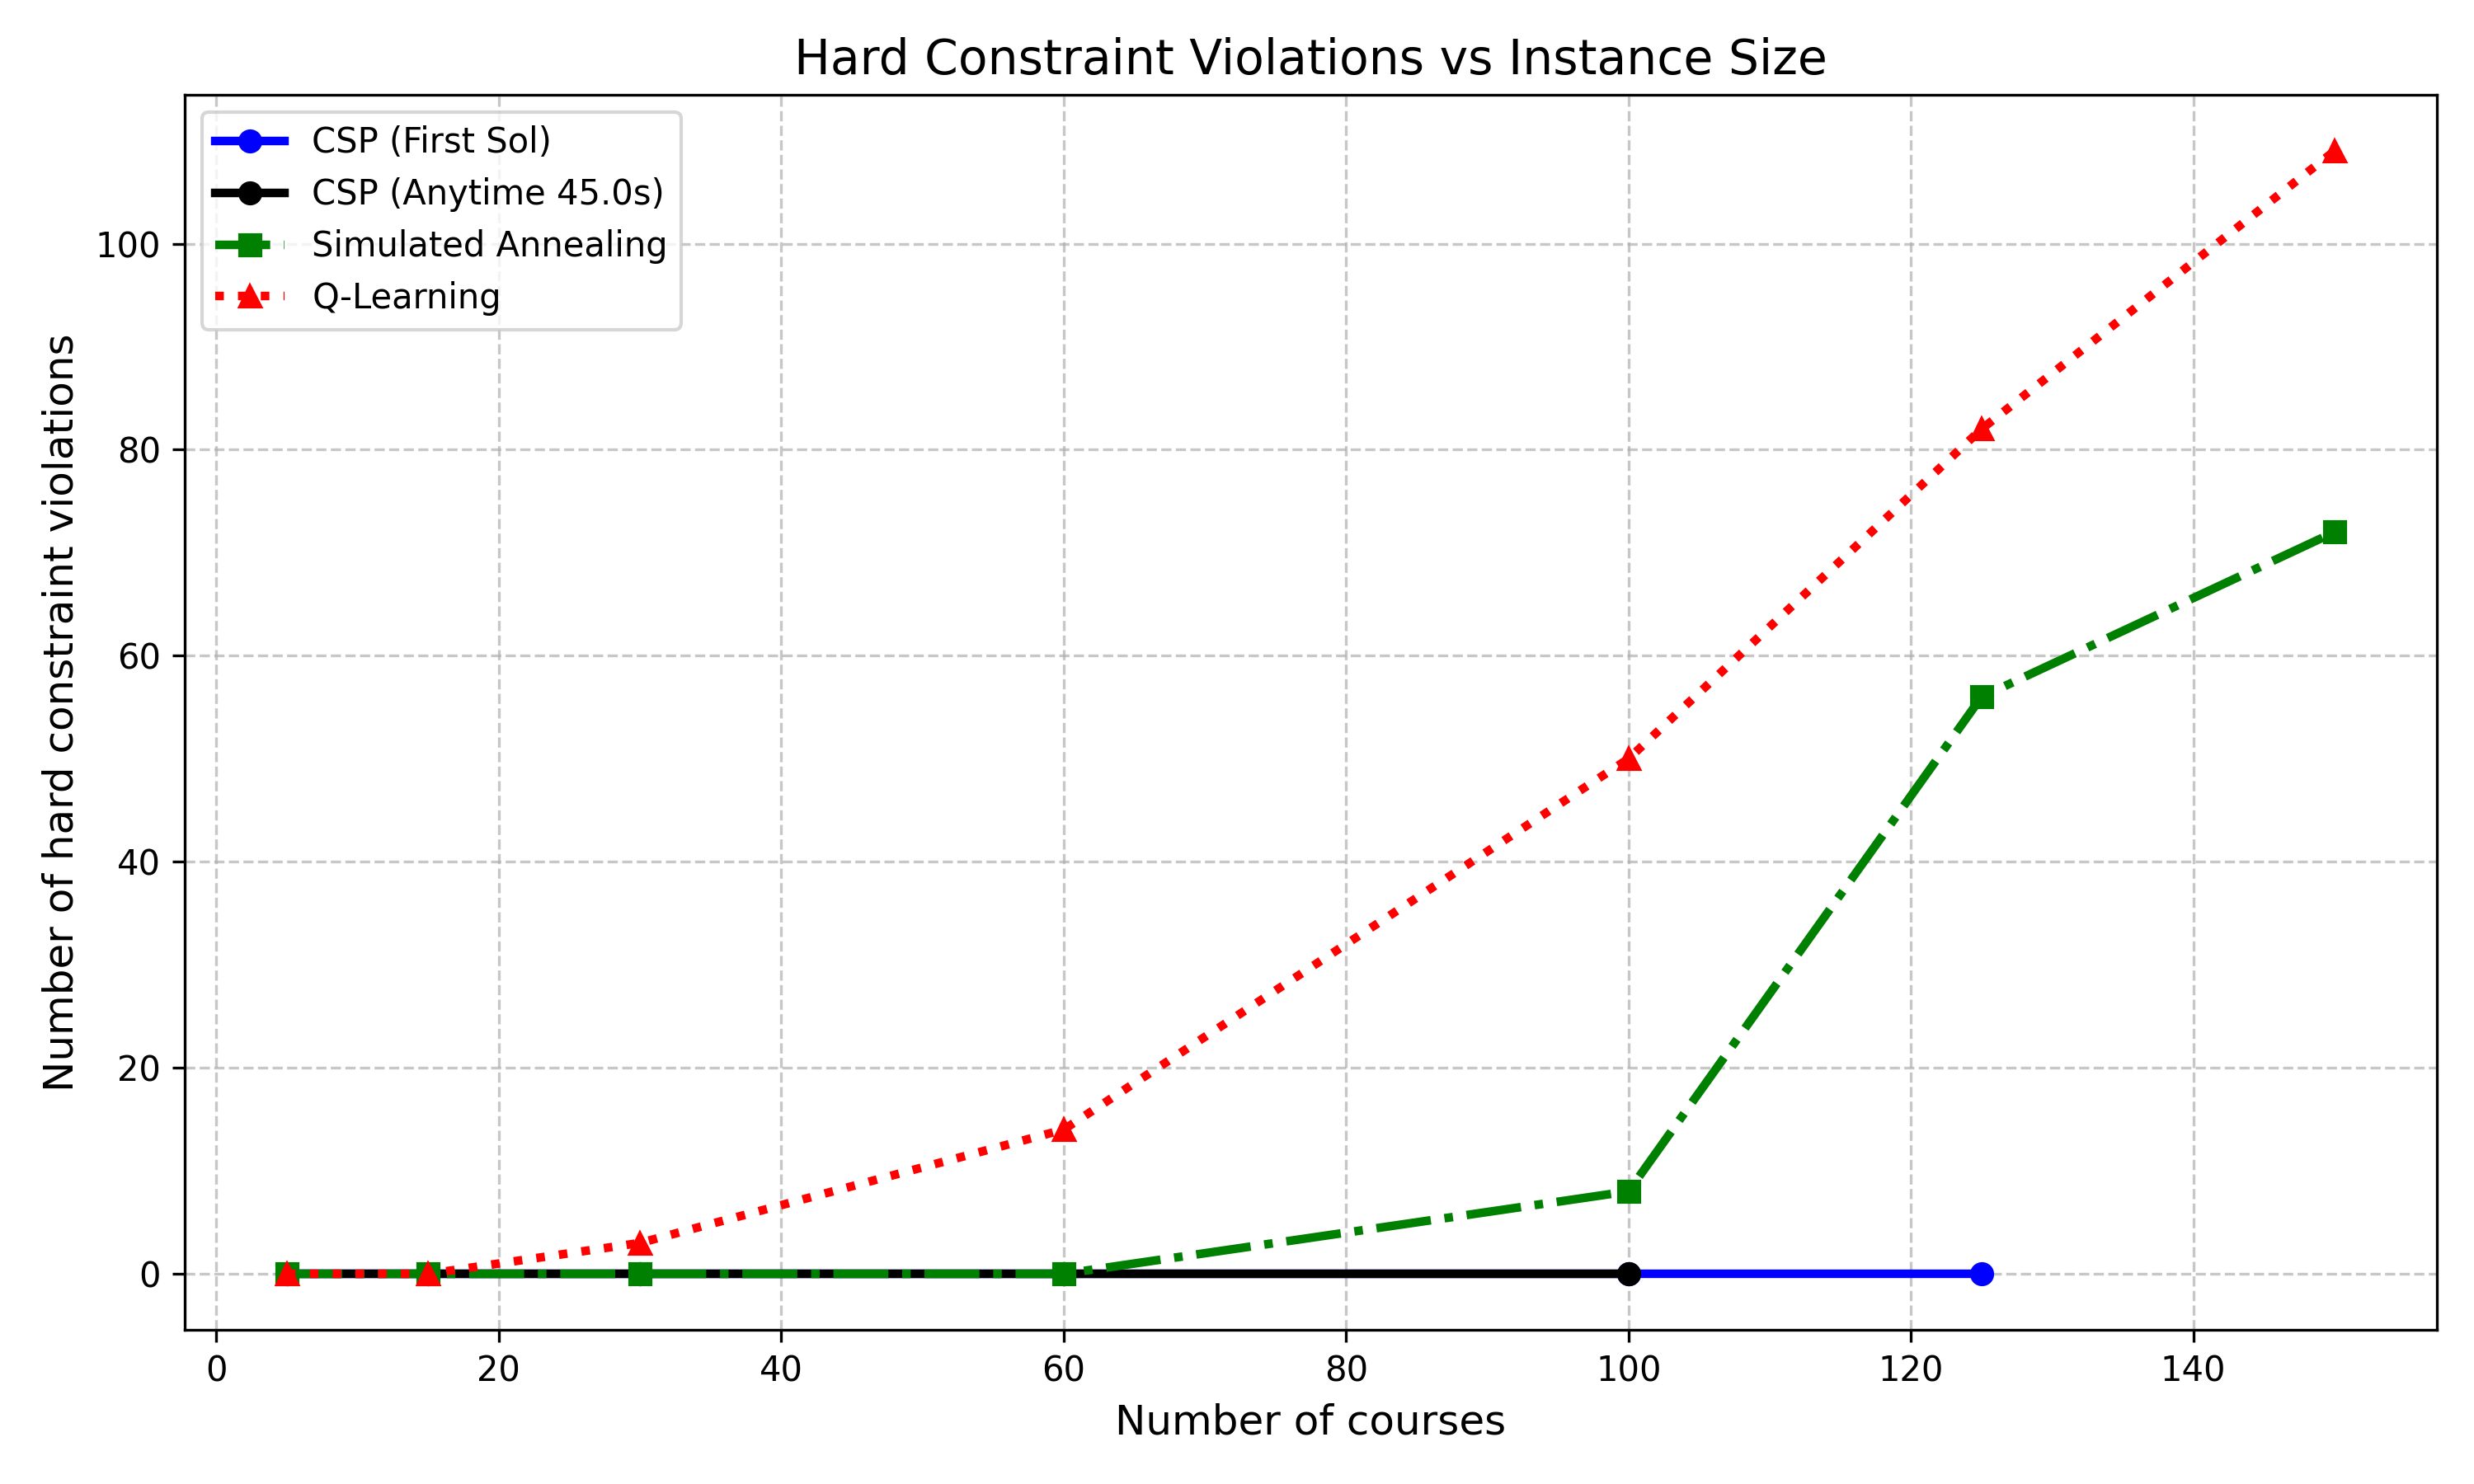
\includegraphics[width=\textwidth]{Images/violations.png}
        \end{column}
        \begin{column}{0.5\textwidth}
            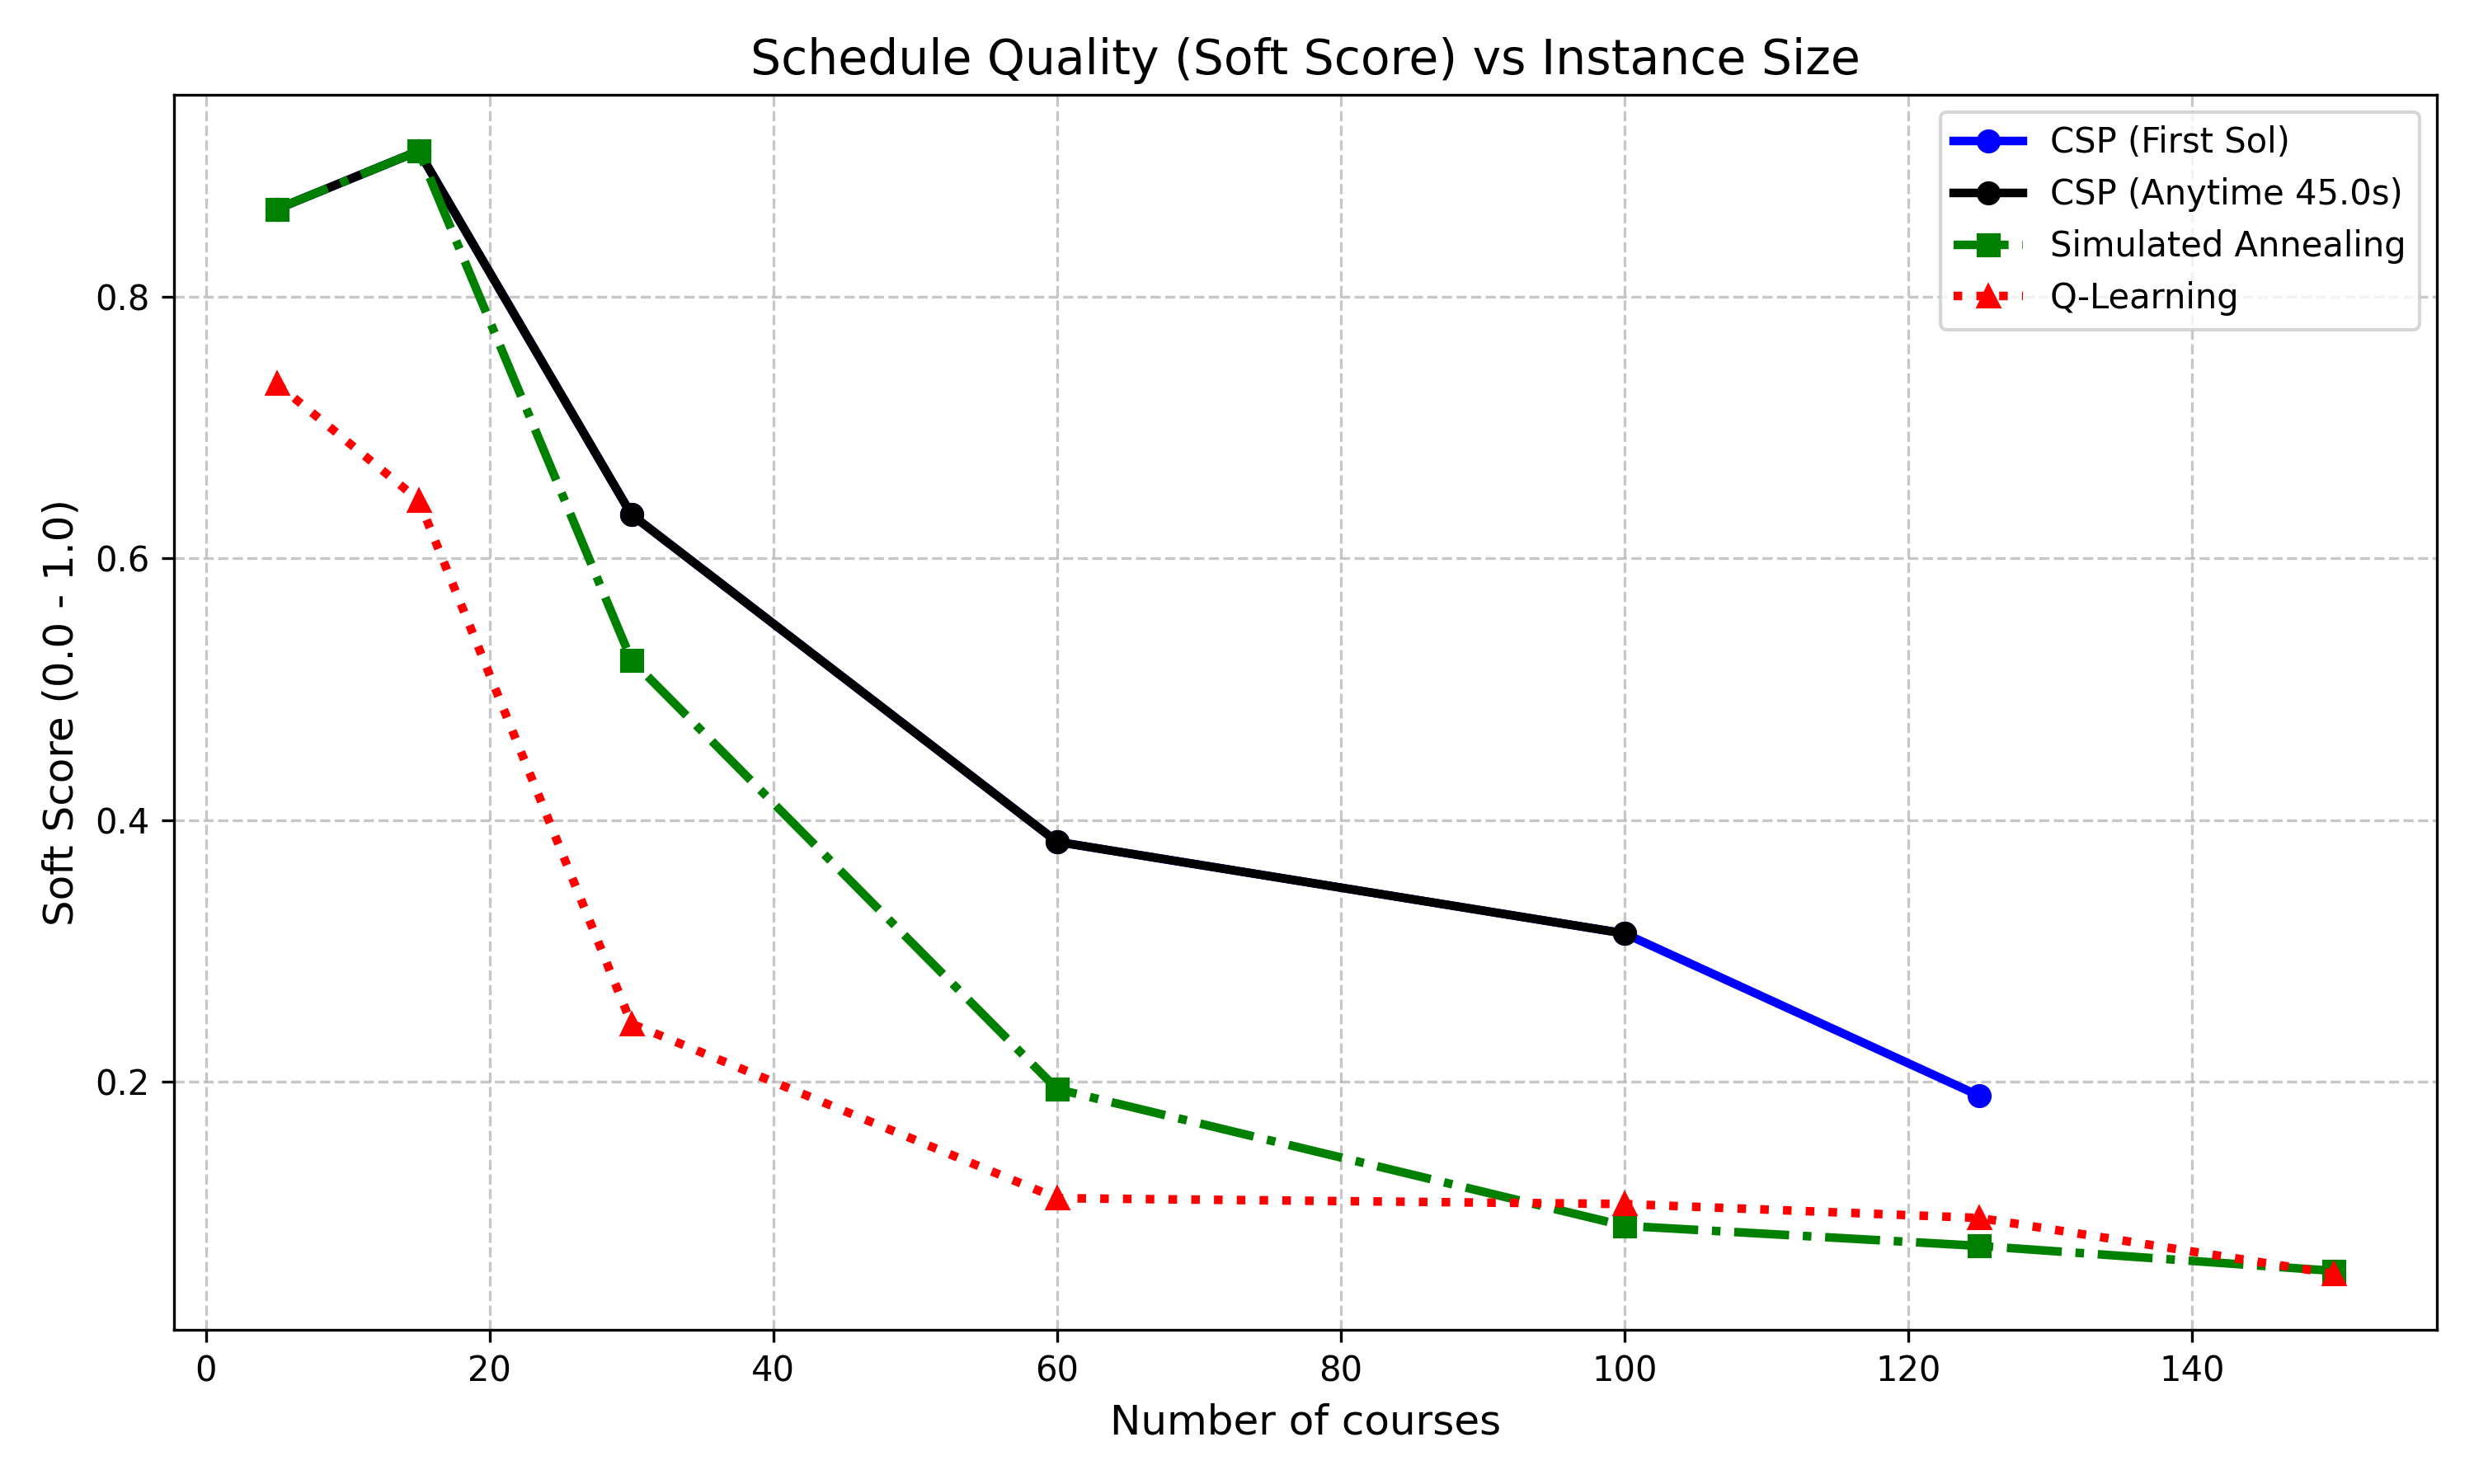
\includegraphics[width=\textwidth]{Images/soft_score.png}
        \end{column}
    \end{columns}

    \bigskip
    \begin{itemize}
        \item \textbf{CSP}: always 0 violations, highest soft score
        \item \textbf{SA}: 0 violations up to 60 courses, soft score drops from $n=60$
        \item \textbf{Q-Learning}: violations explode from $n=30$, soft score collapses
    \end{itemize}
\end{frame}

\begin{frame}{Results: Runtime}
    \begin{center}
        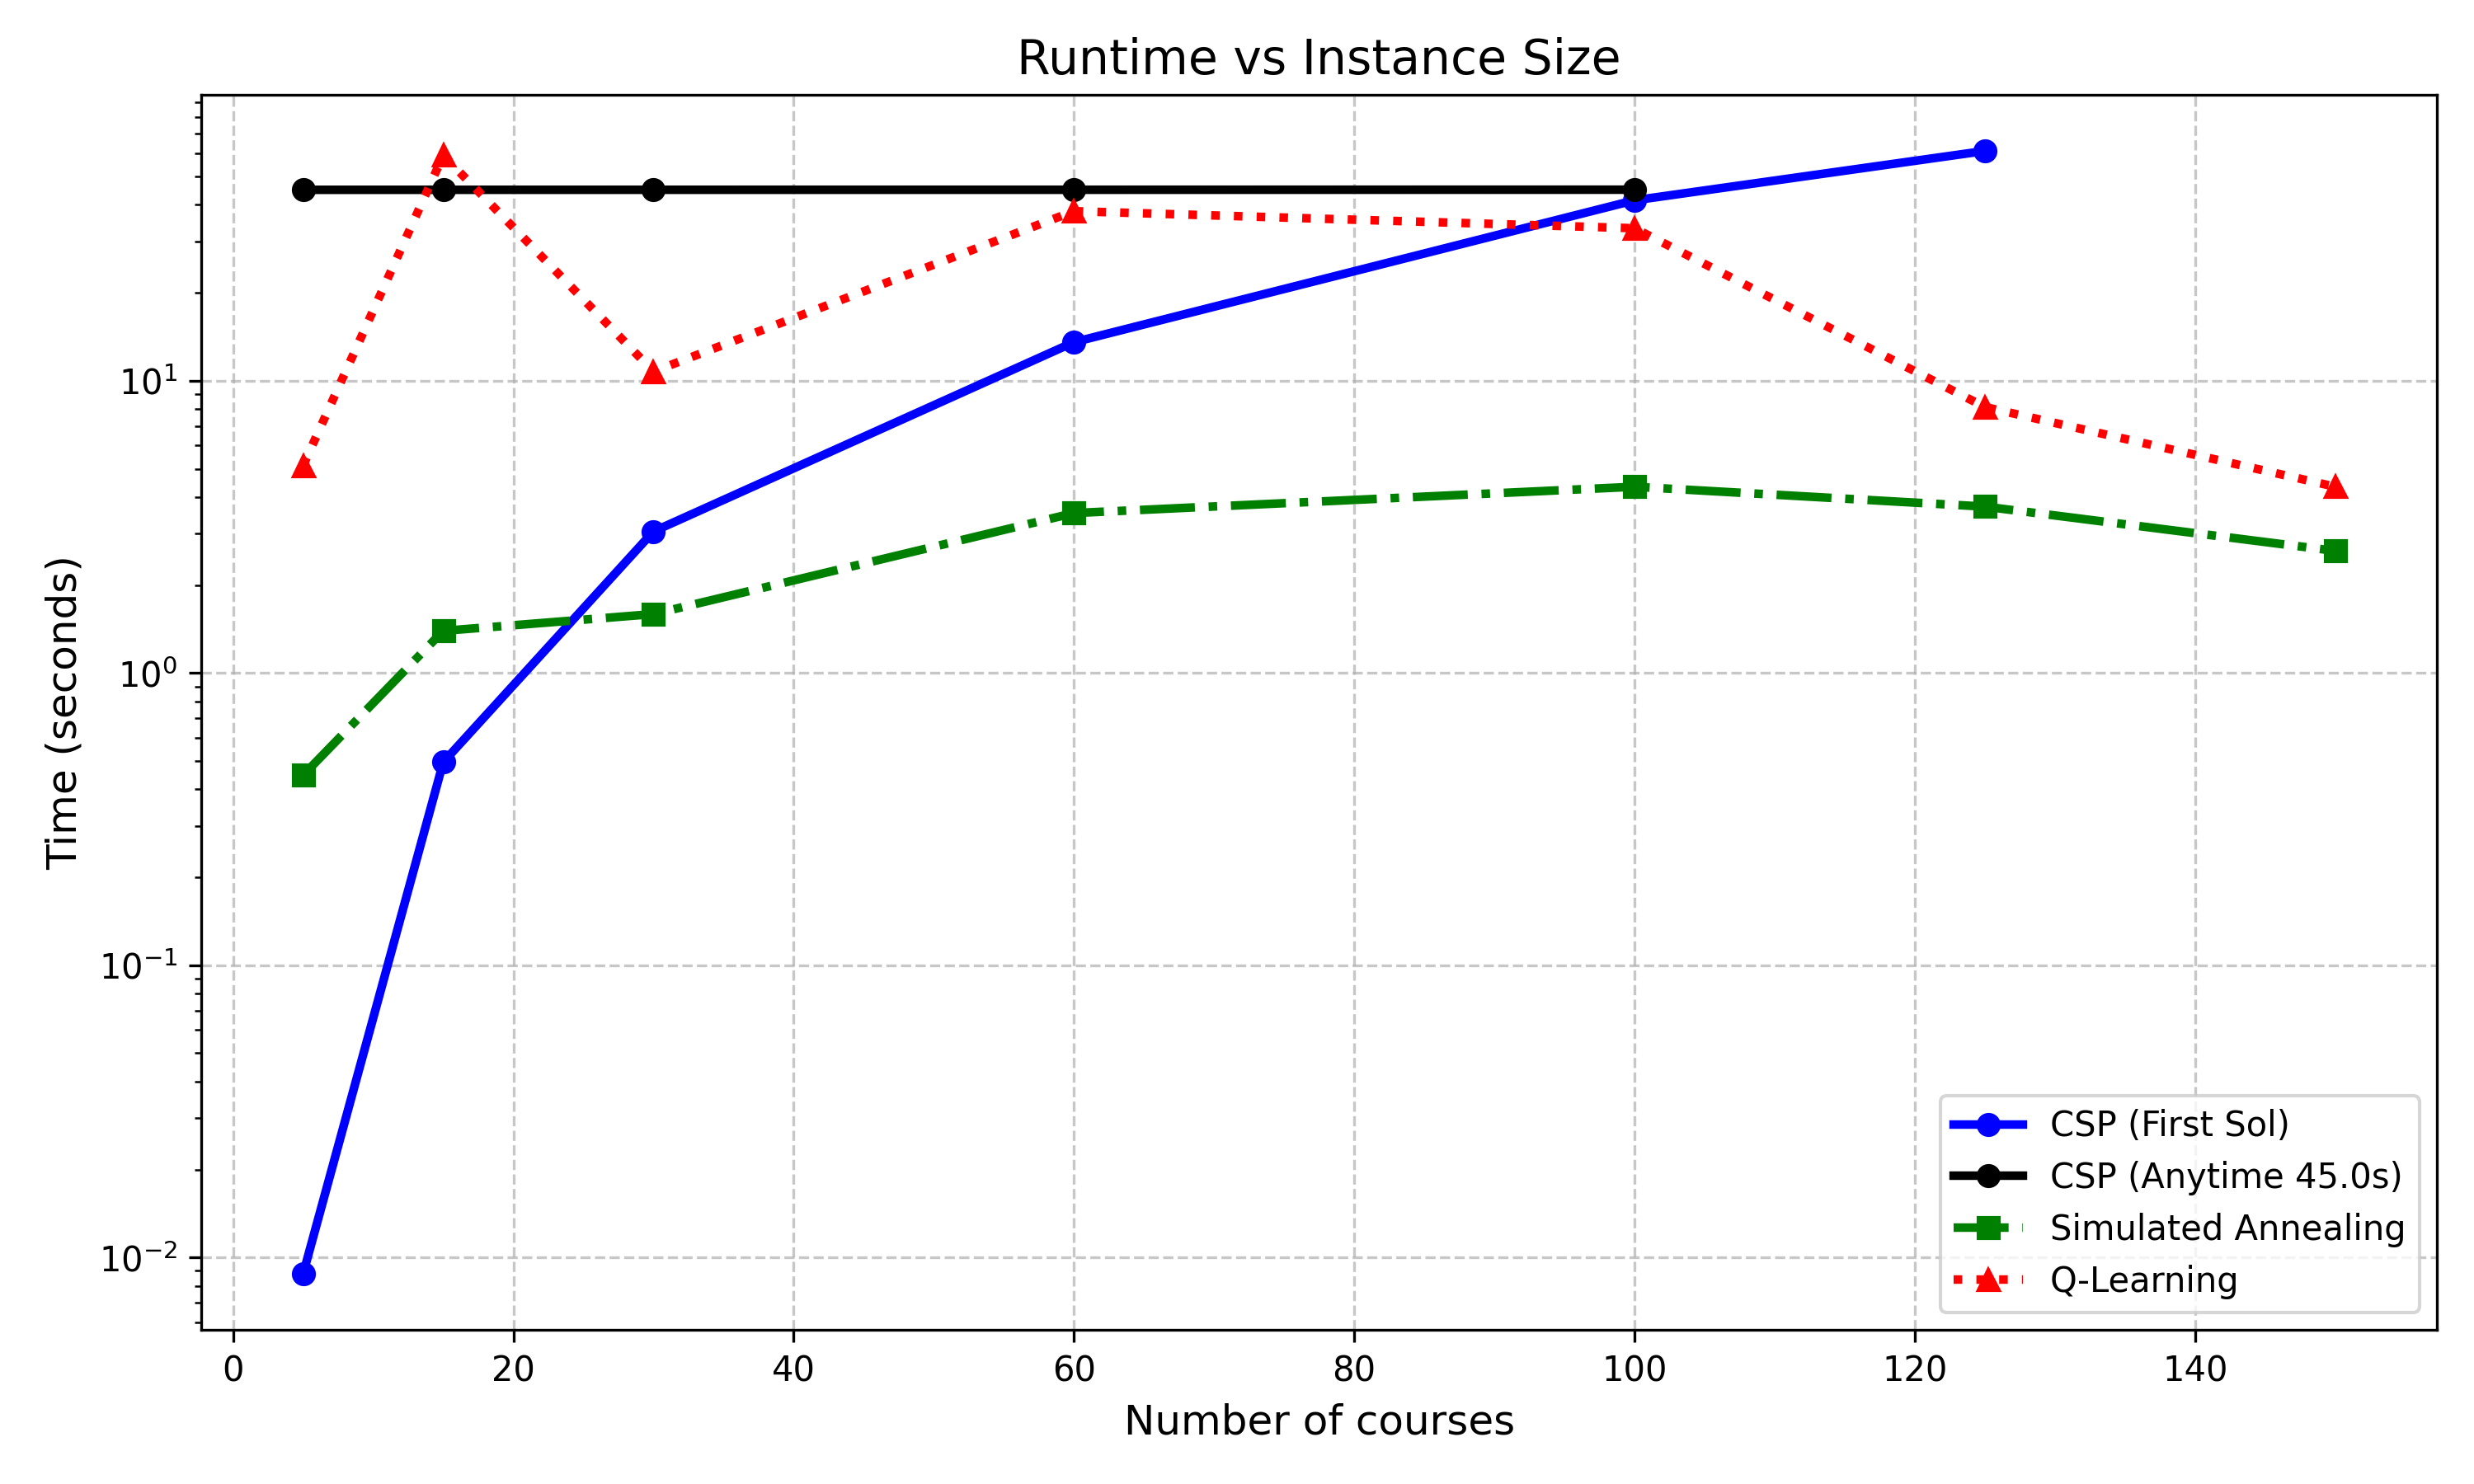
\includegraphics[width=0.75\textwidth]{Images/time.png}
    \end{center}

    \begin{itemize}
        \item \textbf{CSP}: 3\,s at $n=30$ $\to$ 61\,s at $n=125$, hangs at $n=150$
        \item \textbf{SA}: always $< 5$\,s regardless of size
        \item \textbf{Q-Learning}: apparent speed-up on large instances is due to episode truncation (2 episodes), not efficiency
    \end{itemize}
\end{frame}

% -------------------------------------------------------
\section{Conclusion}

\begin{frame}{Qualitative Comparison}
    \begin{table}
    \small
    \begin{tabular}{@{}lccc@{}}
    \toprule
    Criterion        & CSP                & SA              & Q-Learning \\
    \midrule
    Hard violations  & \textbf{Always 0}  & 0 up to 60c     & Grows from 30c \\
    Soft score       & \textbf{Highest}   & Medium          & Low \\
    Scalability      & Fails $>125$c      & \textbf{All sizes} & Poor quality \\
    Predictability   & \textbf{Deterministic} & Stochastic  & Highly variable \\
    Hard guarantee   & \textbf{Yes}       & No              & No \\
    \bottomrule
    \end{tabular}
    \end{table}

    \bigskip
    \begin{block}{Take-away}
        \begin{itemize}
            \item \textbf{CSP} when constraint satisfaction is non-negotiable ($n \leq 125$)
            \item \textbf{SA} as a practical all-round solver for any size
            \item \textbf{Q-Learning} not competitive in tabular form; motivates function approximation or hybrid approaches
        \end{itemize}
    \end{block}
\end{frame}

\begin{frame}[plain]
    \begin{center}
        \Large\textbf{Thank you for your attention}\\[1.5em]
        \normalsize
        Code \& data: \url{https://github.com/BurakSogutlu/Project-TAI-25-26-course_scheduler}
    \end{center}
\end{frame}

\end{document}
